\documentclass{memoria}


\begin{document}

\portada{Informe Entrega 1: Ingeniería de Requerimientos}{Gerson Aguirre Pavez\\Max Chacón Villanueva\\Daniel Gacitúa Vásquez\\Elías González Marincovic \\Nicolás Rozas Sepúlveda}{Profesores: Mauricio Marín Caihuán\\Rodrigo Vásquez Fernández \\ Ayudante: José Orellana}{\today}


\indices

%Introducción (No se incluye en los capítulos del documento)
%-------------------------------------------------------------------------------------
\capitulonn{INTRODUCCIÓN.}

En esta era tecnológica, las redes sociales han formado parte de las relaciones interpersonales, donde se asimila una interacción persona a persona tanto o más natural que en el mundo real. Existen distintas aplicaciones web con distintas funcionalidades para fines específicos dependiendo de los gustos de las personas. Por ejemplo, “Twitter” ofrece una plataforma dinámica de publicaciones con pocos caracteres donde la gente puede expresarse o informarse; “Facebook” permite interactuar con los contactos de manera más amplia, permitiendo publicaciones más extensas, incluyendo fotos, videos, archivos, entre otros; en tanto “Vine” permite subir videos de corta duración para expresar sentimientos, emociones o estados de ánimo.

En esta ocasión, se presenta “BitPhoto”, una plataforma ágil y dinámica que permite a distintos usuarios (profesionales o amateur) cargar fotografías e interactuar entre sus contactos, permitiendo un rápido feedback en sus comentarios. Además, permite localizar de manera geográfica las fotografías cargadas y muestra la información técnica pertinente de cada una de las imágenes, todo esto de manera rápida y actualizada.

Como en todo proceso de desarrollo, se requiere de una planificación previa para organizar los puntos importantes que se deben tomar en cuenta para lograr un resultado exitoso. En un primer acercamiento, se debe conocer y entender las necesidades para buscar una posible solución y de esta manera modelar no solo una solución eficaz, sino también eficiente. En esta primera entrega, la ingeniería de requerimientos será parte fundamental para cumplir con lo anteriormente mencionado, formando la base del desarrollo del producto final.

Para entender las necesidades que se deben cubrir con el software que se desarrollará, se analizarán los requerimientos funcionales y no funcionales, con los cuales se tendrá una idea general de las soluciones que deben plantearse. Posteriormente, se deben asimilar todas estas ideas para comenzar un modelamiento del problema, para esto, se utilizará el modelo de casos de uso y diagrama de clases de análisis, permitiendo una visualización un tanto más concreta de la información obtenida anteriormente.

Luego, en lo que se considera una proyección de lo que será el producto final, se utilizarán los prototipos de la interfaz de usuario, donde se observarán los bocetos de la aplicación web y cómo el usuario va a interactuar con ésta, además de un diseño conceptual de la base de datos para garantizar un funcionamiento óptimo del producto.
 
Todo lo anterior se deberá realizar en un ambiente de trabajo colaborativo del equipo, por lo que se definirán roles de los integrantes y las tareas que éstos deberán realizar. Para que exista una organización y coherencia entre quienes realizan las tareas, es que se trabajará con “Git”, un sistema de control de versiones en el cual se puede observar el trabajo que va haciendo cada integrante del equipo y revisarlo para dar una retroalimentación. Por lo mismo, es importante planificar una estimación de los tiempos en los que se tienen que hacer las distintas tareas y tener un registro para observar el cumplimiento de los deberes y analizar el avance del proyecto en general. Todo lo anterior se realizará con “Trello”, una plataforma interactiva y de fácil usabilidad para el equipo de trabajo, que asemejándose a una carta Gantt, mostrará si el avance en las distintas tareas va de acuerdo a lo propuesto o no.

Con esta entrega se espera tener resuelta la ingeniería de requerimientos, que es quizás, la fase más importante al momento de realizar un proyecto, puesto que constituye la base en la que se trabajará para implementar el resultado final. Con las correcciones que se harán con posterioridad, se comenzará la siguiente fase donde se trabajará la arquitectura para, de esta manera, comenzar a concretar las tareas realizadas en esta oportunidad.   



%-------------------------------------------------------------------------------------
\capitulo{MARCO TEÓRICO.}

\seccion{BASE DE DATOS RELACIONAL.}

Para mayor entendimiento, se define qué es un modelo relacional, el cual es uno de los más empleados a la hora de realizar una base datos, este es un tipo de modelo donde se puede realizar relaciones entre tablas, las cuales son nombradas como entidades y estas a la vez poseen ciertos atributos, los que a través de dichas relaciones se logra una conexión de estos, para a su vez rescatar la mayor información posible de la base de datos.\\

\seccion{DIAGRAMA DE CASOS DE USO.}

Antes de pasar a definir lo que es un diagrama de casos de usos, se debe comprender qué es un caso de uso, el cual puede ser considerado como una receta, debido a que entrega la descripción de los pasos a seguir, también muchas veces mencionado como un camino feliz a lo que se desea realizar, además en un caso de uso se deben manejar ciertas excepciones que pueden ser producidas durante el seguimiento de los ya mencionados pasos.

Luego de ya entender lo que es un caso de uso, se procede a realizar la descripción de qué es un diagrama de casos de usos, partir por definir que éste diagrama es de comportamiento UML. En este diagrama se deben definir los actores y casos de usos, donde se relacionan entre sí, con la idea de que un actor realizará cierto caso de uso, es decir, éste último es considerado una actividad a realizar por cierto actor. Para mayor entendimiento se muestra a continuación como debe ser un diagrama de casos de uso:\\

\begin{figure}[hbtp]
 \centering
 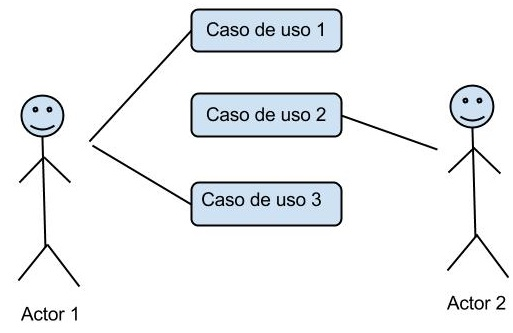
\includegraphics[width=10cm]{MarcoTeorico.jpg}
 \caption{Ejemplo relación Actores/Casos de uso}
 \end{figure}
 
\seccion{DIAGRAMA DE CLASES.}

Es un diagrama que describe un sistema a crear, definiendo qué clases contendrá y que atributos tendrá cada una de estas, es decir, la idea de la creación de un diagrama de clases, es lograr entender de manera ordenada el sistema a crear y así no llegar y programar a tontas y a locas, sino que sabiendo de cierta manera cómo será estructurado el sistema a crear.\\

\seccion{REQUERIMIENTOS FUNCIONALES.}

Este tipo de requerimiento define una funcionalidad del software a realizar o de sus componentes, es decir, establecen el comportamiento del sistema. se recomienda empezar con el usuario puede.\\

\seccion{REQUERIMIENTOS NO FUNCIONALES.}

Es un requisito que especifica ciertos criterios que pueden usarse para juzgar la operación de un sistema en lugar de sus comportamientos específicos. se recomienda empezar estos requisitos con el sistema debe.\\

\seccion{INGENIERÍA DE REQUERIMIENTOS.}

Esta comprende todas las tareas relacionadas con la determinación de las necesidades o de las condiciones a satisfacer para el software a realizar o reconfigurar, tomando en cuenta los requisitos que se relacionan al software correspondiente, esto sea realiza entre las partes interesadas, las que pueden entrar en conflicto entre ellos.



%-------------------------------------------------------------------------------------
\capitulo{ENUNCIADO DEL PROBLEMA.}

Para el proyecto se pide replicar la red social “Flickr”, que su principal objetivo es compartir las fotos de los usuarios y fomentar la retroalimentación mediante las interacciones que la aplicación permite.

Para realizar este trabajo se piden replicar ciertas funcionalidades de las distintas vistas que tiene “Flickr”, las vistas y funcionalidades que se piden son las siguientes:

\begin{itemize}
    \item Vista perfil de usuario: Camera roll, Photo stream, Albums, Map, Favorities y Recent activities.
    \item Vista de personas: Photo from y Photo of.
    \item Vista explorar: Recemt potos, World map y Camera finder.
    \item Vista de búsqueda: Sort, Search y License.
    \item Vista subir imágenes: Add, Remove, Change name, Add tags, Add, people, Add to albums y Owner settings.
\end{itemize}

Para la realización del proyecto se pide conocer y desarrollar el problema con las siguientes tecnologías:

\begin{itemize}
    \item HTML5 en cojunto con AngularJS.
    \item JavaEE y servicios del tipo RESTful.
    \item SOAndroid.
    \item Mysql community edition.
    \item Apache Lucene.
    \item Glassfish.
    \item Gradle.
    \item Weka.
    \item GitHub.
    \item Trello.
\end{itemize}

Para la presente entrega que es la etapa de ingeniería de requerimientos se pide, el listado de requerimientos funcionales y no funcionales, el análisis de los casos de uso y el modelo correspondiente a estos, el diagrama de clases pertinente al problema, un prototipo de interfaz de las diferentes vistas pedidas anteriormente, el diseño conceptual de la base de datos que se utilizará a futuro en la realización del proyecto y la definición de los distintos roles involucrados en la implementación del programa a realizar.


%-------------------------------------------------------------------------------------
\capitulo{MISIÓN Y VISIÓN DEL PRODUCTO DE SOFTWARE.}

\seccion{MISIÓN.}

Nuestra misión como Threads \& Bits Desarrolladores, organización destinada al desarrollo de aplicaciones web y móviles, es  lograr que las personas puedan compartir y hacer del mundo un lugar más abierto y conectado, ofreciendo a nuestros clientes productos de excelencia y con altos estándares de calidad cumpliendo así con sus expectativas y necesidades. Además, consideramos que nuestros clientes son de gran importancia para la organización, por lo cual, nos hemos propuesto entregar productos innovadores, que otorguen soluciones efectivas, seguras, confiables y de alta calidad para responder a las necesidades cambiantes, y contribuir así, a los objetivos particulares de cada uno de éstos, proporcionando de esta manera altos niveles de satisfacción.

Como organización creemos que “BitPhoto” será un producto que cumpla con las expectativas de nuestros clientes, con nuestra aplicación buscamos otorgar una nueva experiencia a las personas, queremos que las personas compartan sus fotografías, sus trabajos, su arte con el mundo, todo esto de manera cómoda, segura y confiable. El ideal de “BitPhoto” es que el usuario tenga la posibilidad de conectarse y comunicarse con todo el mundo, desde amigos o familiares hasta compañeros de trabajo. En conclusión en Threads \& Bits Desarrolladores queremos que Bitphoto se transforme en la red social, para fotógrafos amateurs y profesionales de más éxito a nivel nacional e internacional.


\seccion{VISIÓN.}


Ser una organización multidisciplinaria con el fin de ofrecer soluciones en diversas áreas, integrando la tecnología y principalmente la informática a éstas. Queremos ser una organización que genere confianza en nuestros clientes, y con la sociedad. Que la organización se caracterice por ser una fuente de inversión para el capital humano, permitiéndonos así crear productos de mejor calidad.

A futuro nos vemos como una organización de prestigio y seriedad en el mercado tanto nacional como internacional, logrando así con el tiempo, posicionarnos como un referente nacional en el desarrollo de soluciones informáticas para diversas áreas y campos de la sociedad actual. Queremos llegar a ser un motor que potencie el desarrollo de aplicaciones en nuestro país y latinoamérica, con alta presencia en el mercado internacional, mediante la utilización de tecnología de punta para la creación de nuestros productos. La visión a mediano o largo plazo es poder captar y cautivar a una amplia variedad de clientes, satisfaciendo sus necesidades de manera íntegra y efectiva. Buscamos trabajar con las grandes, medianas y pequeñas empresas en la implementación de soluciones vanguardistas que satisfagan sus necesidades.

Threads \& Bits Desarrolladores tiene como objetivo a corto plazo satisfacer el mercado nacional con la creaciones de nuestro producto “BitPhoto” el cual creemos que nos permitirá crecer y mejorar de manera continua, permitiéndonos de esta manera ampliar el mercado en el cual nos movemos  y mejorar la calidad de los servicios que ofrecemos a nuestros clientes.

Creemos que “BitPhoto” se transformará en la plataforma donde cada fotógrafo profesional o amateur podrá mostrar su trabajo al mundo y conectarse más por medio de las redes sociales.  También tenemos la visión que “BitPhoto” permitirá a organizaciones de distintas índoles mostrar sus actividades por medio de la fotografía. Y creemos firmemente que “BitPhoto” se transformará en la aplicación más utilizada por las personas para almacenar y compartir sus fotografías con familia, amigos, compañeros de trabajo, etc.


%-------------------------------------------------------------------------------------
\capitulo{REQUERIMIENTOS DEL SISTEMA.}

\seccion{REQUERIMIENTOS FUNCIONALES.}

\subseccion{VISTA PERFIL DE USUARIO.}

\textbf{- Camera Roll:}

RF1: El usuario puede ver las fotografías organizadas por fecha, escogiendo por la fecha en que fueron tomadas o la fecha en que fueron cargadas a la aplicación.\\

\textbf{- Photo stream:}

RF2: El usuario puede visualizar las fotografías que ha cargado sin importar si éstas se encuentran en álbumes distintos.

RF3: El usuario puede seleccionar una fotografía cargada para revisar en detalle los datos importantes de ésta (etiquetas, personas que se encuentran en la foto, comentarios, datos técnicos de la cámara, lugar, fecha, cuantas veces ha sido vista y cuantas personas han marcado como favorita la fotografía).

RF4: El usuario puede agregar personas en una fotografía cargada.

RF5: El usuario puede agregar tags o etiquetas a una fotografía cargada.

RF6: El usuario puede comentar una fotografía cargada.

RF7: El usuario puede agregar o mover una fotografía de un álbum a otro.\\

\textbf{- Albums:}

RF8: El usuario puede visualizar los distintos álbumes creados con una de las fotografías que contengan como carátula.

RF9: El usuario puede seleccionar un álbum para visualizar todas las fotografías contenidas en éste.

RF10: El usuario puede crear un nuevo álbum ingresando datos importantes como un nombre, una descripción, y una o más fotografías que ya se encuentren cargadas en la aplicación. \\

\textbf{- Map:}

RF11: El usuario visualiza un mapa del mundo donde puede ubicar de manera geográfica las fotografías que ha cargado, guardándose una dirección donde puede observar la fotografía. 

RF12: El usuario puede buscar una dirección en el mapa. \\

\textbf{- Favorites:}

RF13: El usuario puede visualizar las fotografías de otras personas donde ha marcado la opción “favorito”.\\\\\\

\textbf{- Recent Activity:}

RF14: El usuario puede ver las últimas interacciones relacionadas con actividad en sus fotos, respuestas a sus comentarios en fotos de otras cuentas, notificaciones de seguimiento (follow y followback) y fotos en las que se ha añadido.

RF15: El usuario puede seleccionar un período de tiempo para ver las interacciones que ocurrieron.\\

\subseccion{VISTA DE PERSONAS.}

\textbf{- Photos from:} 

RF16: El usuario puede  ver entre 1 o 5 fotos de las personas a los cuales está siguiendo.\\

\textbf{- Photo of:} 

RF17: El usuario puede visualizar las fotografías en las que se han marcado personas a las que está siguiendo.\\

\subseccion{VISTA EXPLORAR.}

\textbf{- Recent photos:}

RF18: El usuario puede visualizar las fotos recientemente subidas a la aplicación sin importar si sigue o no a las demás personas.

RF19: El usuario puede marcar la opción “favorito” en cualquiera de las fotografías recientes.

RF20: El usuario puede comentar cualquiera de las fotografías recientes.

RF21: El usuario puede ver toda la información técnica de las fotografías recientes.\\

\textbf{- World Map:}

RF22: El usuario puede ver el mapa mundial de fotografías que han sido subidas con ubicación a la aplicación sin importar si está siguiendo o no a las personas.

RF23: El usuario puede seleccionar una marca en el mapa de un lugar específico (país o ciudad) para ver las fotografías localizadas en esa ubicación.

RF24: El usuario puede buscar una dirección, un país o una ciudad  en el mapa, para visualizar todas las fotografías que se han marcado en dicho lugar.\\

\textbf{- Camera Finder:}

RF25: El usuario puede ver las cámaras más populares con las que se han tomado fotografías subidas a la aplicación.

RF26: El usuario puede ver un listado de las distintas marcas de cámaras que se han utilizado.

RF27: El usuario puede ver las especificaciones técnicas de las distintas cámaras, seleccionando un modelo en el listado de cámaras populares.

RF28: El usuario puede visualizar las fotografías que fueron sacadas con una cámara en específico.\\

\subseccion{VISTA DE BÚSQUEDA.}

\textbf{- Sort:} 

RF29: El usuario puede ordenar la búsqueda por orden de relevancia, fotografías recientes o fotografías interesantes.\\

\textbf{- Search:}

RF30: El usuario visualiza las fotografías relacionadas con las palabras clave de su búsqueda.

RF31: El usuario puede filtrar la búsqueda por las fotografías de todos, por sus propias fotografías, por fotografías de sus contactos o usuarios.\\

\textbf{- License:}

RF32: El usuario puede filtrar la búsqueda, mostrándose solo fotografías con permiso comercial, con permiso de modificación, con ambos permisos o fotografías con cualquier tipo de licencias.\\

\subseccion{VISTA SUBIR IMÁGENES.}

\textbf{- Add:}

RF33: El usuario puede arrastrar una o varias fotografías o buscarlas en los directorios de su equipo para cargarla a la aplicación.\\

\textbf{- Remove:} 

RF34: El usuario puede remover una o varias fotografías que hayan sido seleccionadas para ser cargadas a la aplicación.\\ 

\textbf{- Change name:}

RF35: El usuario puede cambiar el nombre de una o varias fotografías que hayan sido seleccionadas para ser cargadas a la aplicación.\\

\textbf{- Add tags:}

RF36: El usuario puede agregar variadas etiquetas o tags a una o varias fotografías que hayan sido seleccionadas para ser cargadas a la aplicación.\\

\textbf{- Add people:}

RF37: El usuario puede agregar distintas personas en una o varias fotografías que hayan sido seleccionadas para ser cargadas a la aplicación.\\

\textbf{- Add to albums:}

RF38: El usuario puede agregar una o varias fotografías, que hayan sido seleccionadas para ser cargadas a la aplicación, a distintos álbumes sin importar si estos ya ha existen o deben crearse.\\

\textbf{- Owner Settings:}

RF39: El usuario puede escoger la licencia que desee para una o varias fotografías que hayan sido seleccionadas para ser cargadas a la aplicación.\\

\subseccion{VISTA INICIAR SESIÓN.}

RF40: El usuario puede ingresar sus datos de registro para iniciar sesión.

RF41: El usuario puede mantener sus sesión iniciada mediante la opción “Recordar sesión”.\\


\seccion{REQUERIMIENTOS NO FUNCIONALES.} 

RNF1: La aplicación deberá estar disponible para teléfonos móviles con sistema operativo Android (4.0 IceCream Sandwich de Android o superior).

RNF2: La aplicación Web debe usar la tecnología AngularJS.

RNF3: La forma de persistir la información del sistema será mediante una base de datos relacional ocupando el gestor de base de datos MySQL.

RNF4: La base de datos debe ofrecer soporte a datos geoespaciales.

RNF5: El sitio web del sistema debe utilizar HTML5 para sus vistas.

RNF6: El sistema debe someter a análisis los comentarios de los usuarios del sistema, con el fin de analizar sentimientos (positivo,negativo,neutral) mediante la herramienta WEKA.

RNF7: El sistema debe implementar un motor de búsqueda mediante la indexación de tags y comentarios, utilizando la  herramienta APACHE Lucene.

RNF8: El sistema debe permitir geolocalizar fotografías.

RNF9: El sistema debe utilizar JEE para la creación del web service de tipo RestFul.

RNF10: La aplicación tanto web como móvil tendrá su interfaz en español latino.

RNF11: La aplicación debe poseer un diseño web adaptativo (\textsl{Responsive Web Design}).

RNF12: La aplicación web debe desplegarse en los navegadores web Chrome (versión 35 o superior), Firefox (versión 30 o superior), Opera (versión 20 o superior), Safari(versión 7 o superior), Internet Explorer (versión 9 superior).

RNF13: La base de datos del sistema debe ser alimentada por medio de la API de Flickr.

RNF14: El sistema debe velar por la privacidad de sus usuarios, el sistema no puede divulgar información que los usuarios no han autorizado.

RNF15: La aplicación Web y Móvil debe permitir identificar en todas sus vistas el nombre o icono de “Bit Photo”.

RNF16: La aplicación web y móvil debe indicar al usuario en qué instancia se encuentra.

RNF17: La aplicación web y móvil deberá estar habilitada 24 horas al día y los 7 días de la semana de manera regular.

RNF18: La aplicación se debe desarrollar utilizando el lenguaje de programación Java con algunas características de la versión JEE con las tecnologías CDI, JPA, EJB, JAX-RS.

RNF19: El servidor de aplicaciones que el sistema debe usar es GlassFish.

RNF20: El sistema debe señalar errores de la aplicación o de ejecución al usuario.

RNF21: En caso de falla de un componente del sistema no debe haber pérdida de información.

RNF22: El sistema entregará información actualizada de los usuarios y sus imágenes en  el sistema.

RNF23: Los formatos de fotografías permitidos por la aplicación serán JPEG y PNG no animado.

RNF24: La cantidad de fotografías soportadas por álbumes en el sistema será de 20 fotos.

RNF25: La aplicación tanto web como móvil deben señalar al usuario las condiciones de privacidad y uso de datos del usuario.

RNF26:La aplicación web debe indicar al usuario que componentes del dispositivo se utilizarán para la aplicación, y debe solicitar permiso para su uso.

%-------------------------------------------------------------------------------------
\capitulo{CASOS DE USO.} 

\seccion{LISTADO DE CASOS DE USO.}

Los casos de uso que se pueden identificar a partir de los requerimientos funcionales y de las funcionalidades que requiere el sistema, son los siguientes:

\begin{enumerate}
    \item Revisando historial de fotografías cargadas.
    \item Revisando fotografías cargadas.
    \item Revisando álbumes creados.
    \item Visualizando mapa de fotografías cargadas.
    \item Editando localización de fotografías cargadas.
    \item Visualizando fotos marcadas como favoritos.
    \item Visualizando actividad reciente de otros usuarios.
    \item Visualizando fotos de usuarios a quienes se está siguiendo.
    \item Visualizando fotografías en las que se han marcado personas a las que se está siguiendo.
    \item Visualizando fotografías recientemente cargadas a la aplicación.
    \item Visualizando mapa mundial de fotografías cargadas.
    \item Visualizando cámaras que se han utilizado con la aplicación.
    \item Buscando palabras clave.
    \item Subiendo imágenes.
    \item Interactuando con fotografías cargadas.
\end{enumerate}
\newpage
\seccion{DIAGRAMA DE CASOS DE USO.}

Se ha identificado solamente un actor que interactúa con el sistema utilizando las funcionalidades que se han especificado anteriormente. El usuario de la aplicación se ha denominado "Usuario BitPhoto", y el modelo de casos de uso se presenta a continuación:\\

\begin{figure}[hbtp]
 \centering
 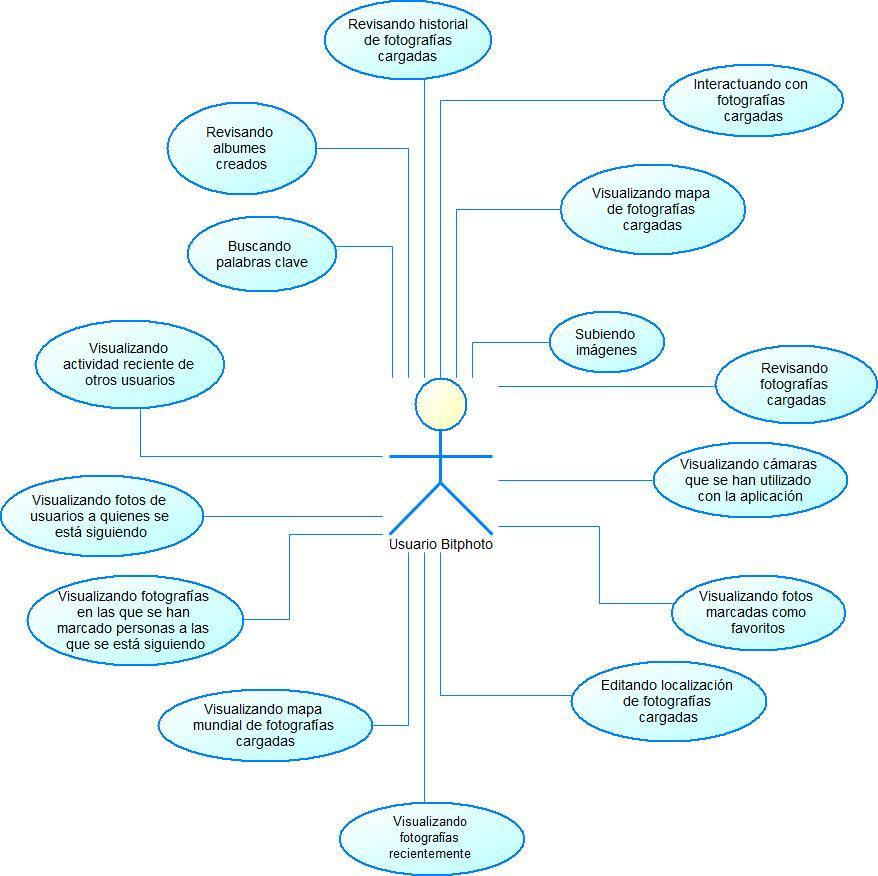
\includegraphics[width=15cm]{DiagramaDeCasosDeUso.jpg}
 \caption{Diagrama de Casos de Uso}
 \end{figure}
  

%-------------------------------------------------------------------------------------
\capitulo{DIAGRAMA DE CLASES DE ANÁLISIS.}



%-------------------------------------------------------------------------------------
\capitulo{PROTOTIPO DE INTERFAZ DE USUARIO.}

%-------------------------------------------------------------------------------------
\capitulo{BASE DE DATOS.}

%-------------------------------------------------------------------------------------
\capitulo{GESTIÓN DEL PROYECTO.}
    

\end{document}
